\documentclass[a4paper,12pt]{article}

\usepackage{rotating}
\usepackage[top=1in, bottom=1in, left=0.75in, right=0.75in]{geometry}
\usepackage{graphicx}
\usepackage[numbers,square,sort&compress]{natbib}
\usepackage{setspace}
\usepackage[cdot,mediumqspace,]{SIunits}
\usepackage{caption}
\usepackage{subcaption}
\usepackage{mathtools}
\usepackage{authblk}
\usepackage{float}
\renewcommand{\thesubsection}{\thesection.\alph{subsection}}
\providecommand{\e}[1]{\ensuremath{\times 10^{#1}}}

\begin{document}
\onehalfspacing
\title{PHY 407 Lab 3}
\author{Natalie Price-Jones, 999091021}
\date{3 October 2014}
\affil{\small{natalie.price.jones@mail.utoronto.ca}}
\maketitle

\section{Question 1}

\subsection{Part b)}

The solution to

\[
\left[ \begin{array}{cccc}
0 & 1 & 4 & 1\\
3 & 4 & -1 & -1\\
1 & -4 & 1 & 5\\
2 & -2 & 1 & 3
\end{array} \right]
\mathbf{x} = 
\left[ \begin{array}{c}
-4 \\ 3 \\ 9 \\ 7
\end{array}\right],
\]

is given by 

\[
\mathbf{x} = \left[ \begin{array}{c}
 1.61904762 \\ -0.42857143 \\ -1.23809524 \\ 1.38095238
\end{array}\right]
\]

\section{Question 2}

\subsection{Part c)}

The Hamiltonian has the following energy eigenvalues for the first ten eigenstates: $E_0 = 5.84 eV$, $E_1 = 11.18eV$, $E_2 = 18.66 eV$, $E_3 = 29.14 eV$, $E_4 = 42.65 eV$, $E_5 = 59.18 eV$, $E_6 = 78.72 eV$, $E_7 = 101.27 eV$, $E_8 =   126.83 eV$, $E_9 = 155.53 eV$. These values also appear in Table \ref{tab:energy} below.

\subsection{Part d)}

\begin{table}[H]
  \centering
  \begin{tabular}{|c||c||c||c|}
  \hline
  Energy State & H is $10 \times 10$ & H is $100 \times 100$ & Residual\\
  \hline
  \hline
   $E_0$ & 5.83605892708 & 5.83605852627 & $4.00801756228\e{-7}$\\
	\hline
	 $E_1$ & 11.1801874046 & 11.1801860811 & $1.32348002246\e{-6}$\\
	\hline
	 $E_2$ & 18.6608447561 & 18.6608428848 & $1.87132323148\e{-6}$\\
	\hline
	 $E_3$ & 29.1405379677 & 29.1405291667 & $8.8010350936\e{-6}$\\
	\hline
	 $E_4$ & 42.6493457585 & 42.6493366369 & $9.12161883093\e{-6}$\\
	\hline
	 $E_5$ & 59.1770021258 & 59.1769495345 & $5.25913648133\e{-5}$\\
	\hline
	 $E_6$ & 78.7181197916 & 78.7180679555 & $5.18361046034\e{-5}$\\
	\hline
	 $E_7$ & 101.270800354 & 101.27016932 & 0.000631034660444\\
	\hline
	 $E_8$ & 126.832800525 & 126.831967988 & 0.000832536703854\\
	\hline
	 $E_9$ & 155.532402483 & 155.402760328 & 0.129642155138\\
	\hline
  \end{tabular}
  \caption{}
\label{tab:energy}
\end{table}

As can be easily seen in Table \ref{tab:energy}, using 10 or 100 as the side length for H matters very little for the low eigenvalues. However, as you go to higher energies, the eigenvalues computed become more different between the side lengths at an approximately exponential rate. This exponential behaviour is more obvious in Figure \ref{fig:q2d}, where the y-axis has been log scaled.

\begin{figure}[H]
\centering
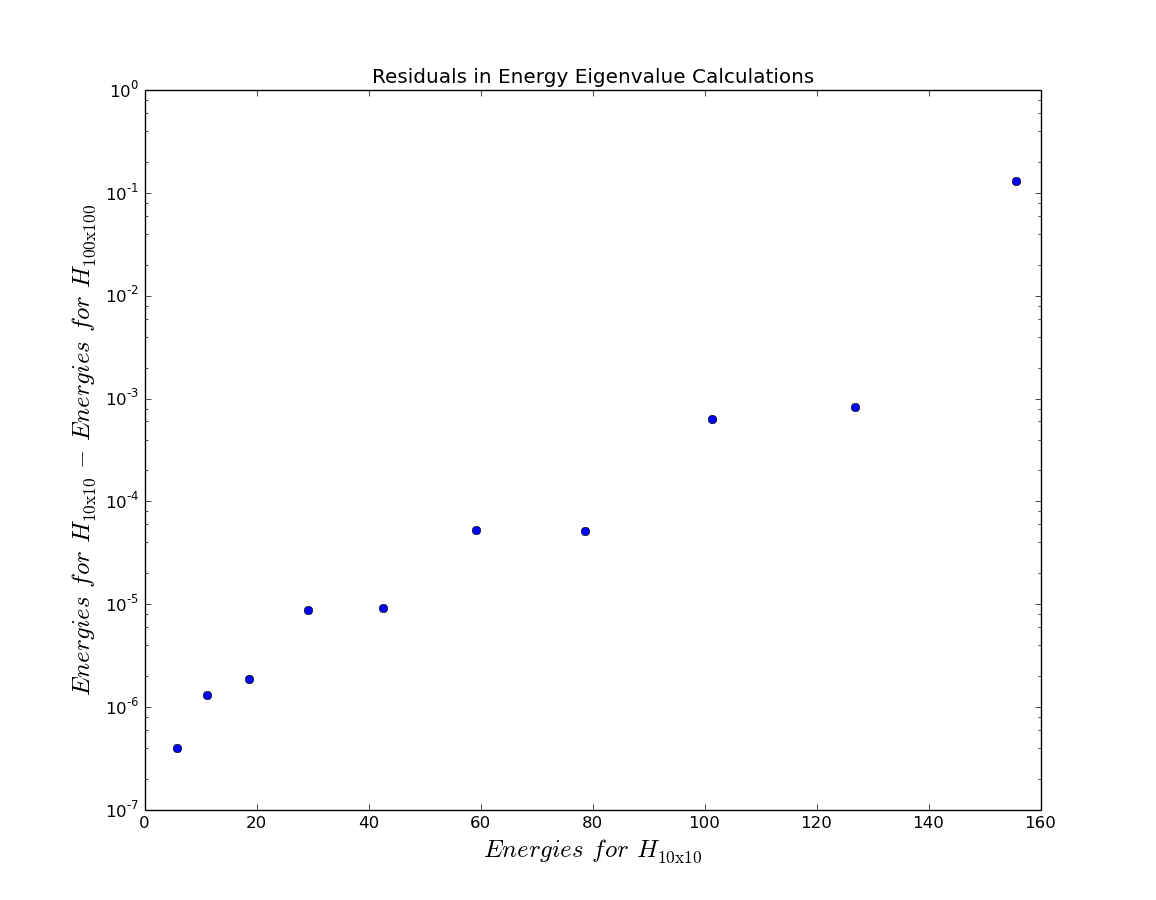
\includegraphics[width = \linewidth]{lab4q2d.png}
\caption{}
\label{fig:q2d}
\end{figure}

In short, the higher you go in energy, the more terms you need in your Hamiltonian for accurate results.

\subsection{Part e)}

\begin{figure}[H]
\centering
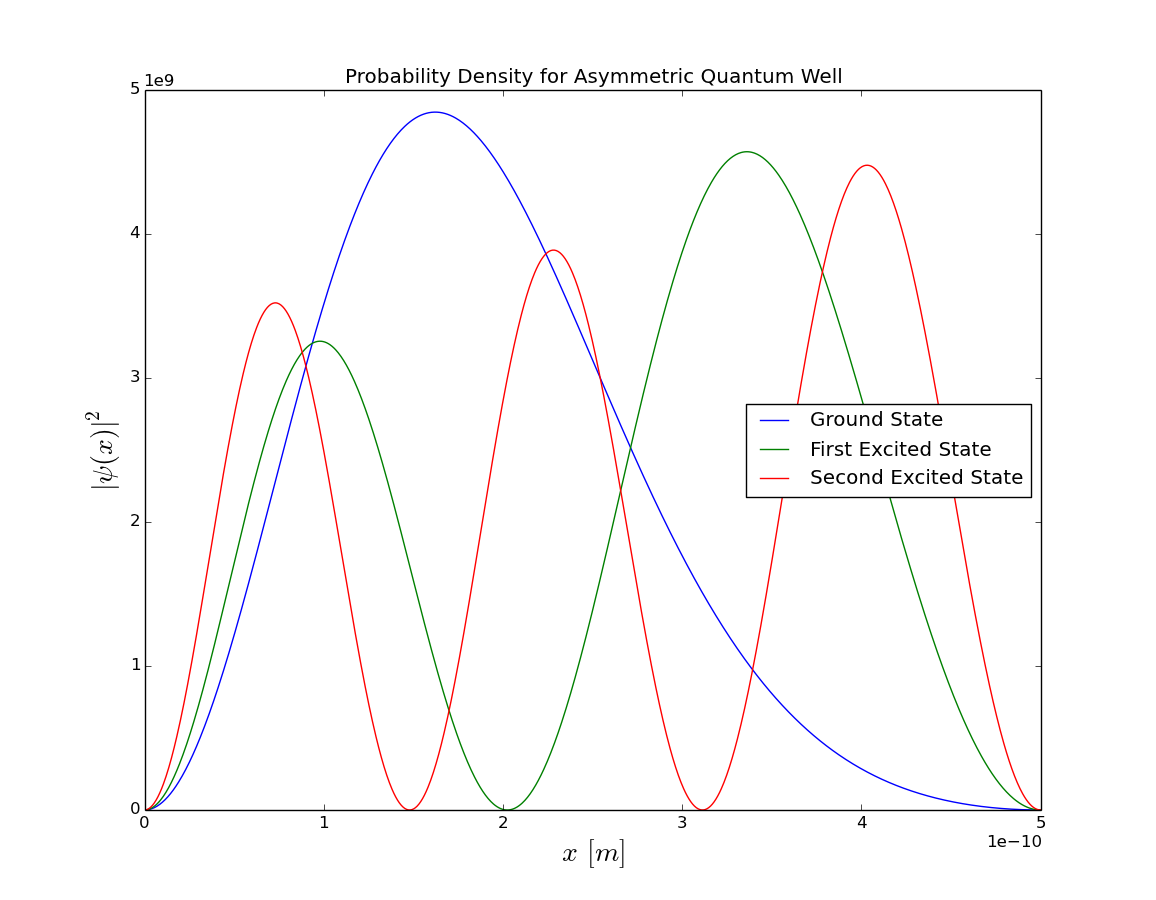
\includegraphics[width = \linewidth]{lab4q2ef.png}
\caption{Normalized probability density functions for the ground state and the first two excited states. The probability density is quite high because the scale of the well is so small (on the order of a nanometre). This normalization was done manually; since the eigenvector solutions had arbitrary magnitudes it was necessary to rescale them after computation.}
\label{fig:q2ei}
\end{figure}

\section{Question 3}

\subsection{Part a)}

The solution to $x = 1 - e^{-cx}$ when $c = 2$ is $x = 0.796813$.

\subsection{Part b)}

\begin{figure}[H]
\centering
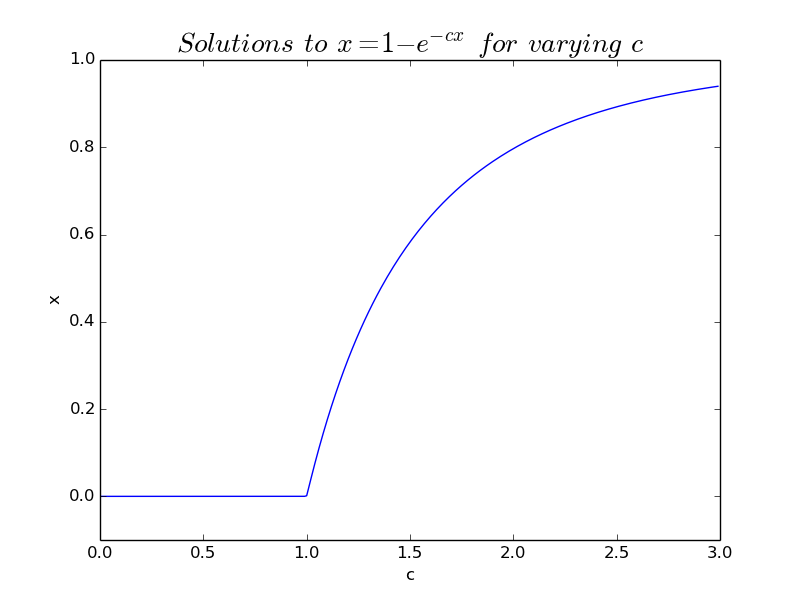
\includegraphics[width = \linewidth]{lab4q3b.png}
\caption{}
\label{fig:q3}
\end{figure}

\section{Question 4}

\subsection{Part a)}

We can show that the error in the overrelaxation method ($\epsilon '$), subject to some approximations, is given by:

\begin{eqnarray}
\epsilon'\simeq \frac{x-x'}{1 - 1/[(1+\omega)f'(x)-\omega]},\label{eqn:eps}
\end{eqnarray}

where $x'$ is the current solution, $x$ is the previous solution, $f(x)$ is the function equal to $x$ we are attempting to solve and $\omega$ is the parameter of the over relaxation.

We start with the definition of $x'$ for the over relaxation and the algebra follows from there.

\begin{eqnarray}
x' &=& x + (1+\omega)\Delta x = (1+\omega)f(x) - \omega x\nonumber\\
x' &=& (1+\omega)(f(x^*) + (x-x^*)f'(x^*) + ...) - \omega x \mathrm{\:\:\:(Taylor\;expand\;f(x))}\nonumber\\
x' &\simeq & (1+\omega)(x^* + (x-x^*)f'(x^*)) - \omega x \mathrm{\:\:\:(Drop\; higher\;order\;terms\;and\;use\;}x^* = f(x^*)\mathrm{)}\nonumber\\
x' &\simeq & x^* + \omega \epsilon - (1+\omega)\epsilon f'(x^*) \mathrm{\:\:\:(Used\;} x^* = x + \epsilon\mathrm{\;to\; rewrite\;} x^*-x)\nonumber\\
-\epsilon' &\simeq& \epsilon (\omega - (1+\omega)f'(x))\mathrm{\:\:\:(Used\;} x^* = x' + \epsilon' \mathrm{\; as\; above\; and\;} f'(x^*)\simeq f'(x)\mathrm{\; near\;} x^*)\nonumber\\
\implies \epsilon &\simeq& \frac{\epsilon'}{(1+\omega)f'(x) - \omega}\nonumber
\end{eqnarray}

Now substitute the expression for $\epsilon$ into $x^* = x + \epsilon$.

\begin{eqnarray}
x^* &\simeq& x + \frac{\epsilon'}{(1+\omega)f'(x) - \omega}\nonumber\\
x' + \epsilon' &\simeq& x + \frac{\epsilon'}{(1+\omega)f'(x^*)-\omega} \mathrm{\:\:\:(Since\;} x^* = x + \epsilon = x' + \epsilon')\nonumber\\
\epsilon'\left(1 - \frac{1}{(1+\omega)f'(x) - \omega}\right) &\simeq& x - x'\nonumber\\
\epsilon' &\simeq& \frac{x-x'}{1-1/[(1+\omega)f'(x) - \omega]}\nonumber 
\end{eqnarray}

So under the assumptions that $f(x)$ is well approximated by the first two terms of its Taylor series and that $f'(x^*)\approx f(x)$ near $x^*$, we have shown that Equation \ref{eqn:eps} is a good approximation of the uncertainty in the value $x'$ with respect to the true value.x

\subsection{Part c)}

When using over relaxation with $\omega = 0.72$, the result converged to the required accuracy in 3 iterations. Without this over relaxation, getting the required accuracy required 13 iterations. Some alternate guesses were made for $\omega$, but $0.72$ provided the most improvement over the regular relaxation method.

\subsection{Part d)}

In the over relaxation method ($x' = (1+\omega)f(x) - \omega x$ for $\omega > 0$), the $\omega$ parameter causes a controlled overshooting in each iteration. Under relaxation takes place when $\omega < 0$, and this approache undershoots each iteration. This approach is more useful than over relaxation in when $f(x)$ is not well behaved near our solution for $x$. In particular, if the value of $f(x)$ blows up near the solution, approaching the solution slowly is better than over shooting and landing on a vertical asymptote. In addition, if there are multiple solutions to $x = f(x)$, an appropriate initial guess and under relaxation ensures the right solution is found.


\section{Question 5}

The following equation is satisfied by the $r =$ the $L1$ Lagrange point:

\begin{eqnarray}
\frac{GM}{r^2} - \frac{Gm}{(R-r)^2} &=& \omega^2r\nonumber\\
\implies \frac{GM}{r^2} - \frac{Gm}{(R-r)^2} - \omega^2r &=& 0
\label{eqn:lag}
\end{eqnarray}

Where $G$ is the gravitational constant, $M$ is mass of the Earth, $m$ is the mass of the Moon, $R$ is the distance between the Earth and the Moon and $\omega$ is the angular velocity of the Moon about the Earth.

The calculated value of the $L1$ Lagrange point using the secant method is $3.260\e{8}$ m. Setting $r = L1$ means Equation \ref{eqn:lag} evaluates to $3.579\e{-6}$, which is certainly close to zero.

\section{Question 6}

The effeciency $\eta$ of an incandescent bulb at a particular temperature $T$ is given by:

\begin{eqnarray}
\eta = \frac{15}{\pi^4}\int_{hc/\lambda_2 k_B T}^{hc/\lambda_1 k_B T} \frac{x^3}{e^x - 1} dx,\nonumber
\end{eqnarray}

where $h$ is Planck's constant, $c$ is the speed of light in a vacuum, $k_B$ is the Boltzmann constant, $\lambda_1 = 390$ nm and $\lambda_2 = 750$ nm.

\subsection{Part a)}

\begin{figure}[H]
\centering
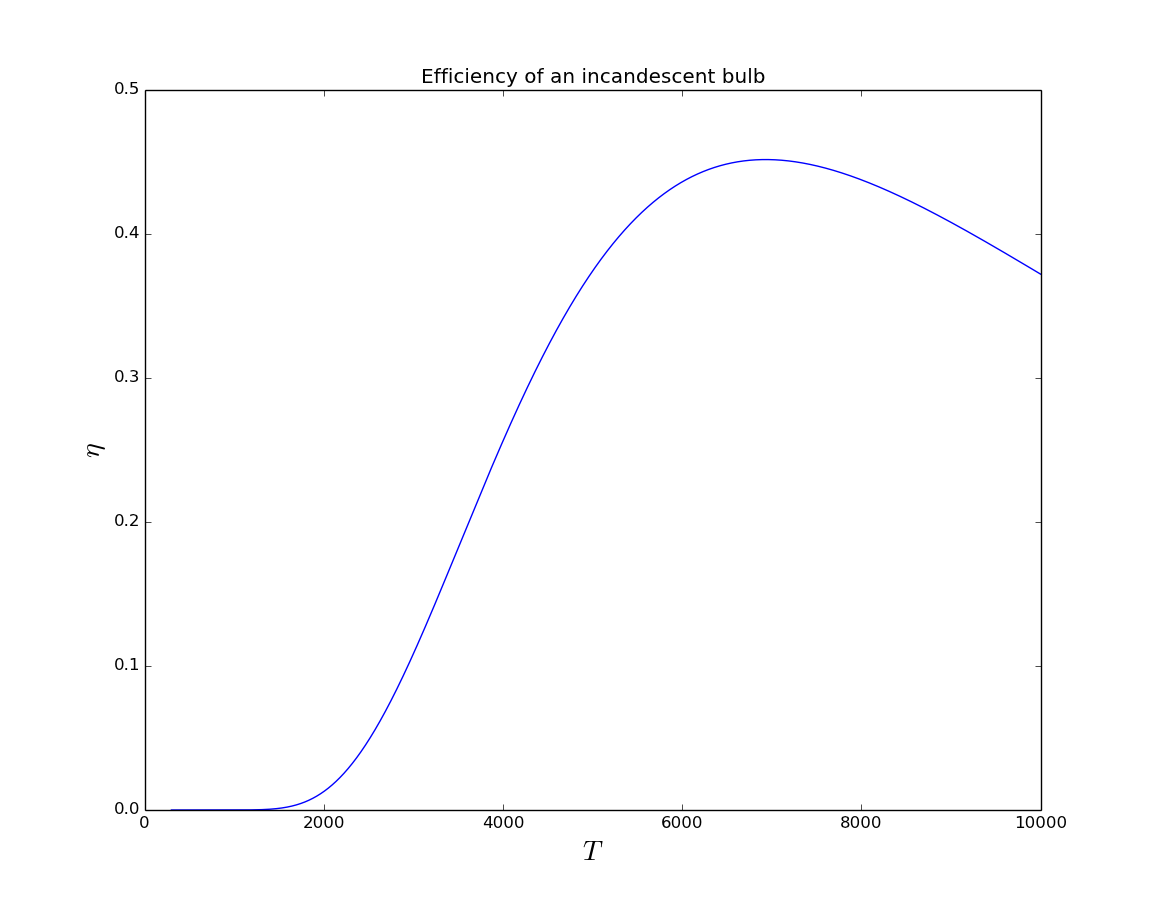
\includegraphics[width = \linewidth]{lab4q6a.png}
\caption{}
\label{fig:q6}
\end{figure}

\subsection{Part b)}

The maximum efficiency in Figure \ref{fig:q6} above occurs at $T = 6933.2087415$ K.

\end{document}





